\chapter{Localization Algorithm} \label{chap:pf}
Our solution is based on \acl{MCL}, introduced in chapter~\ref{chap:fundamentals}. Figure~\ref{fig:algo_architecture} provides an architectural overview of our solution, including the involved sensors and components.

In this chapter we first outline the reasons for choosing \acs{MCL} instead of another algorithm. Next we describe the algorithms \emph{motion model}, which is on one side responsible for tracking the users motion by combining different sources, introduced in chapter~\ref{chap:sensors}, and on the other side for the sampling from the motion model. Afterwards, we give a detailed insight in our solution's \emph{measurement model}. It tracks the beacon's signals, resp.\ the distances to the beacons, and implements the \acs{PF}'s importance factor calculation. In the end, we explain the algorithm's implementation, which builds upon the motion and measurement model.

\begin{figure}
\def\svgwidth{0.9\textwidth}
\input{algo_architecture.pdf_tex}
\caption{Architecture}
\label{fig:algo_architecture}
\end{figure}


\section{Design Decision} \label{sec:algo_decision}
As mentioned in chapter \ref{chap:fundamentals}, there are different approaches for indoor localization. Our approach is based on \acl{PF}, resp.\ \acl{MCL}, due to the following reasons.

As shown in chapter \ref{chap:ibeacons} and mentionend by \citet{IEEE:survey_wireless_indoor_pos}, wireless signals are heavily influenced by obstacles and the environment, thus we decided not to just rely on the measured distances to the beacons. As outlined in chapter \ref{chap:sensors}, smartphone usually include sensors, such as an accelerometer, gyroscope, and a magnetometer, which can be used to estimate, for instance, a walked distance. Consequently, the algorithm needs to be able to fuse the different sensor data, to improve the location estimation by reducing its uncertainty, which is one of the main reasons for choosing \acs{PF}.

As depicted by \citet{siddiqi:experiments_mcl_wifi} and \citet{wang:wlan}, using the map information additionally to the sensor fusion drastically improves location accuracy. For example, particles resp.\ location hypothesizes, wich are out of bound or not accessible by the person can be weed of \citep{straub:pf,siddiqi:experiments_mcl_wifi}. Sensor fusion would also be possible by using a \acl{KF}, resp.\ \acs{EKF}, but according to \citet{wang:wlan}, ``distributed information like the map information is impossible to be integrated for tracking by \acs{EKF}'', which is the second main point for choosing \acs{PF}.

Another advantage of \acs{PF}, compared to \acs{KF}, is its ability of solving the \emph{global localization problem}. It gives the algorithm the possibility to recover form failure state, e.g.\ if the estimated location is completely wrong, due to short-term sensor failure, which is a important feature.

Compared to other approaches, \acs{PF} has the advantage of taking uncertainties into account, which the other mentioned algorithms, except \acs{KF}, do not. \acs{KF} is just able to model uncertainties in form of gaussians. As mentioned before, \acs{PF} is a non-parametric filter, thus it has the advantage of providing the location estimation in form of a multi-modal posteriori belief, which can be visually expressed very well, as depicted in \ref{fig:pf_approx}, which can be a benefit for the user.

As stated out in chapter \ref{chap:intro}, the requirements of our solution are, a small pre-deployment effort and a simple and cheap infrastructure to reduce the cost of purchase and the ongoing maintenance costs. By using \acs{PF}, based on \acs{RSS} distance estimation and additional build-in sensors, less pre-deployment effort is required, compared to scene analysis approaches, which need an additional time consuming offline stage. Compared to other solutions, e.g.\ the acoustic localization approach proposed by \citet{hoflinger:acoustic}, our infrastructure requirements are very low. The user just requires a capable smartphone, and the building just needs to be equipped with \emph{cheap} beacons. Their, system requires specific hardware with microphones which are being connected with each other. Also the smartphone needs a connection to the measuring unit which is responsible for the location estimation in their solution, or at least, to receive the measurements.

Besides the above mentioned reasons, \acl{PF}, resp.\ \acs{MCL}, is an easy-to-implement algorithm with is additionally a well-known and well-studied localization algorithm in robotics, as mentioned by \citet{thrun:prob_robo}, which is able to do landmark based localization, as requested in indoor self-localization with smartphones using iBeacons.

\section{Motion Model}\label{sec:algo_motion_model}
Our solution's motion model component is responsible for three tasks, firstly, for tracking the users motion, secondly, to determine if the user is stationary, and thirdly, to allow the \acs{PF} to sample from the motion model. The three tasks are prerequisites for our \acs{PF}'s implementation.

\subsection{Motion Tracking}
As mentioned in chapter~\ref{chap:sensors}, iOS's CoreMotion framework provides a component called \texttt{CMPedometer}, which estimates distances based on the steps a user has taken. In addition, the CoreLocation framework provides the device heading, based on the magnetic field, called \texttt{CLHeading}. Furthermore, CoreMotion's \texttt{CMDeviceMotion} provides the device \texttt{attitude}, which is being calculated by using sensor fusion. The device's attitude can also be to also calculate the device heading. By combining these three sources, the user's motion can be tracked, and a path can be constructed.

\paragraph{Heading}
As mentioned in chapter~\ref{chap:sensors}, the heading provided by \texttt{CLHeading} can be influenced by other magnetic fields than the earth's magnetic field, which may cause wrong values. \texttt{CMDeviceMotion}, which relies not just on the magnetometers values, by using sensor fusion, is not being influenced by other magnetic fields, but against the claims made by Apple's engineers, the values tend to drift away \citet(?). Thus, using just the \texttt{CMDeviceMotion.attitude} is also not sufficient. Consequently, we combine both sources to determine the heading.

Both frameworks do provide their values asynchronously. \acs{CL} calls its delegate method if a certain threshold of the heading's change exceeds, which we set to $1^\circ$. Whereas, \acs{CM} calls its delegate periodically, which we set to $50 Hz = 0.02 sec$. The high update rate would not be necessary for the heading, but as mentioned earlier \texttt{CMDeviceMotion} does also include \texttt{userAccleration}, which is being used for the stationary detection, as shown later.

The \texttt{CMDeviceMotion} heading, further denoted as $\theta_A$, measured at time $t$, is being calculated from the rotation matrix, given by \texttt{CMDeviceMotion.attitude}, as explained in chapter~\ref{chap:sensors}. Due to its drift problem just the change, denoted as $\Delta\theta_A$ between two values is being used. For the absolute orientation, \texttt{CLHeading.magneticHeading}, denoted as $\theta_C$, is being used. Internally, the motion tracking uses the heading $\theta$, which also takes the map's orientation $\theta_M$ into account. $\theta$ is being calculated if \acs{CL}'s heading filter is being exceeded and thus, a new magnetic heading is being provided, but not if \acs{CM} provides a new $theta_A$ due to its high update frequency, which would result in lots of updates of $\theta$ with very small change.

Figure~\ref{lst:mm_heading} illustrates the used algorithm to combine the two heading sources to calculate the internally used heading $\theta$, for more robustness against the influence of disturbing magnetic fields, without the drift problem. Furthermore, figure~\ref{tab:mm_heading} provides a calculation example for better understanding.

\begin{figure}
\begin{lstlisting}[mathescape]
// instance variables
$\theta_{A_\text{current}}$, $\theta_{A_\text{last}}$ = nil
$\theta_{C_\text{last}}$ = nil

// combined internal heading
$\theta$ = 0.0

// called by CoreMotion if new heading is available
didMeasureDeviceMotionHeading($\theta_{A_t}$) {
  $\theta_{A_\text{current}} = \theta_{A_t} - \theta_M$
}

// called by CoreLocation if new heading is available
didMeasureCompassHeading($\theta_{C_t}$) {
  $\theta_{C_\text{current}} = \theta_{C_t} - \theta_M$
  
  if $\theta_{A_\text{latest}} \neq \text{nil}$ && $\theta_{A_\text{last}} \neq \text{nil}$ && $\theta_{C_\text{last}} \neq \text{nil}$ {
    $\Delta\theta_{A} = \theta_{A_\text{current}} - \theta_{A_\text{last}}$
    $\Delta\theta_{C} = \theta_{C_\text{current}} - \theta_{C_\text{last}}$
    
    $\theta_{A_\text{last}} = \theta_{A_\text{current}}$
    
    $\theta = \theta_{t-1} + \frac{\Delta\theta_{C} + \Delta\theta_{A}}{2}$
  } else {
    $\theta = \theta_{C_\text{current}}$
  }
  
  $\theta_{C_\text{last}} = \theta_{C_\text{current}}$
}
\end{lstlisting}
\caption{Illustrates the calculation of the internal heading $\theta$, by combining $\theta_C$ and $\theta_A$, relative to the maps orientation $\theta_M$}
\label{lst:mm_heading}
\end{figure}

\begin{figure}
\begin{tabular}{c|ccc|c|ccc||c}
\textbf{$t$} & \textbf{$\theta_C$} & \textbf{$\theta_A$} & \textbf{$\theta_M$} & $\theta_{C_\text{current}}$ & $\theta_{C_\text{last}}$ & $\theta_{A_\text{current}}$ & $\theta_{A_\text{last}}$ & \textbf{$\theta$}\\
\hline
$t_0$ & $90.3$ & & $20.0$ & $70.3$ & & & & $70.3$\\
$t_1$ & & $78.2$ & $20.0$ & & $70.3$ & $58.2$ & &\\
$t_2$ & & $79.0$ & $20.0$ & & $70.3$ & $59.0$ & $58.2$ &\\
$t_3$ & $91.3$ & & $20.0$ & $71.3$ & $70.3$ & $59.0$ & $58.2$ & $71.2$\\
$t_4$ & & $79.7$ & $20.0$ & & $71.3$ & $59.7$ & $59.0$ &\\
$t_5$ & $92.3$ & & $20.0$ & $72.3$ & $71.3$ & $59.7$ & $59.0$ & $72.1$\\

\end{tabular}
\caption{Example illustrating the calculation of the internal heading $\theta$, according to the algorithm depicted in figure~\ref{lst:mm_heading}}
\label{tab:mm_heading}
\end{figure}

\paragraph{Motion Path Construction}
As explained in chapter~\ref{chap:sensors}, \acs{CM} delivers every $\sim 2.5\text{sec}$ a new \texttt{CMPedometer} object with the estimation of the distance $d$ a user traveled. Besides the distance the object contains the start date $t_\text{start}$, which is the start date of the very first distance estimation, which is the same for all successive estimations. Additionally, it contains the $t_\text{end}$ date. Thus the user walked a estimated distance $d$ beginning at $t_\text{start}$ and ending at $t_\text{start}$.
During the walk, the user's direction $\theta$ changes several times at a certain point in time, denoted with $t$.

A user's motion path is being stored as an array of motions $u$. A motion consists of $u = (\theta, d, t_\text{start}, t_\text{end})^T$, the orientation $\theta$ at the motions start date $t_\text{start}$, the distance $d$ in meters and the motions end date $t_\text{end}$. $t_\text{start}$ and $t_\text{end}$ are not really necessary for constructing the estimated motion path, but are necessary for the later explained importance factoring.

To calculate the motion $u$ of a walked distance $d$, the distance is being split up according to the timestamps corresponding to the orientational changes, which occurred during the estimated distance. Therefor, constant velocity over the distance $d$ is being assumed. Figure~\ref{fig:mm_path} illustrates the estimated path a user traveled in 2-dimensional space. The individual distances $d_1, d_2$, estimated by \acs{CM}, are colored differently. By integrating the measured headings $\theta_0, \ldots, \theta_4$, the path is split up in motion $u_0, \ldots, u_5$.


\begin{figure}
	\begin{tikzpicture}
	  \draw[->] (0,0) -- (8,0); 
  	  \draw[->] (0,0) -- (0,7);
  	  \draw (8.5,0)node(y){$x$};
  	  \draw (0,7.5)node(y){$y$};
  	  
  	  
  	  \draw[blue] (1,6)--(5,6);
  	  \draw (1,6.5)node(a){$\theta_0$};
  	  \draw[blue] (3,6.5)node(b){$d_0$};
  	  \draw(3,5.5)node(b){$u_0$};
%  	  \fill[red] (5,6) circle (2pt);
  	  
  	  \draw[blue] (5,6)--(7,4);
  	  \draw (5,6.5)node(c){$\theta_1$};
  	  \draw(5.6,4.7)node(b){$u_1$};
  	  
  	  \draw[blue] (7,4)--(7,3);
  	  \draw (7.5,4)node(d){$\theta_2$};
  	  \draw(6.5,3.5)node(b){$u_2$};
  	  
  	  \draw[red] (7,3)--(7,1);
  	  \draw (7,0.5)node(e){$\theta_3$};
  	  \draw(6.5,2.0)node(b){$u_3$};

  	  \draw[red] (7,1)--(3,1);
  	  \draw[red] (5,0.5)node(b){$d_1$};
  	  \draw(5,1.5)node(b){$u_4$};
  	  
  	  
  	  \draw[red] (3,1)--(3,4);
  	  \draw (3,0.5)node(e){$\theta_4$};
  	  \draw(3.5,2.5)node(b){$u_5$};
  	    	  
  	  
  	  
	\end{tikzpicture}
\caption{Illustration of motion path construction, by integrating heading $\theta_0, \ldots, \theta_4$ into the two estimated walked distances $d_1, d_2$. $u_0, \ldots, u_5$ depict the resulting motions.}
\label{fig:mm_path}
\end{figure}


\subsection{Stationary Detection}\label{sec:algo_stationary}
As mentioned in chapter~\ref{chap:sensors}, iOS \texttt{CMPedometer} component requires at the beginning approx.\ 6--8 steps to deliver the first distance estimation. During a walk it continuously updates the estimation every $\sim 2.5\text{sec}$. Due to the asynchronous incoming motion and \acs{BLE} measurement data, the filter cannot be run continuously, with a fixed time interval, because the later discussed measurements need to be integrated at the right position on the users walk. Therefor, it is important to know if the user is currently walking resp.\ is stationary or not.

\citet{wang:wlan} proposes a system based on acceleration data to detect a users steps by detecting the acceleration's zero-crossing. Whereas we do not actually need to count the users steps, this approach needs to much effort. \citet{shanklin:embedded_sensors} use the acceleration data to also estimate the distance the user traveled but they just integrate the values two times to get the distance, with a preceding low pass filter. Thus, for our implementation integration of the acceleration would be sufficient enough to get the user's velocity, which could be used to determine the users stationary state. Therefor, the a projection of the measured acceleration data into the global coordinate system is required, as also described in their work. Unfortunately, their solution, worked very unreliable. According to \citet{wang:wlan}, integration of acceleration data for distance estimation does just work in theory, but not reliably in indoor environment. Furthermore, their proposed projection is being based on \texttt{CMDeviceMotion}'s \texttt{attitude} property, because they also used an iOS device, which has the drift problem.

But, \citet{shanklin:embedded_sensors} also considered another solution for step detection which uses the user's minimum acceleration, which is being detected by using a threshold that needs to be exceeded by the acceleration's Euclidian-Norm $\left\lVert a \right\rVert$, shown in equation~\ref{eq:a}. Figure~\ref{fig:mm_stationary_1} depicts the user's 3-axis acceleration during a walk with two, clearly visible, stops. The corresponding Euclidian-Norm is being shown in figure~\ref{fig:mm_stationary_2}. For the actual detection of the stationary and not stationary state, we added a simple moving average, which is being calculated over the last $50$ values, resp.\ by $50\text{Hz}$ the last second. If our threshold of $\left\lVert a \right\rVert > 0.1 ms^{-2}$ is exceeded the user is walking, if not, the user is stationary.

The solution's advantage is, that it is quite easy to implement and does not need a projection of the acceleration data. As a result, the later discussed integration of measurements, resp.\ the importance factoring can be delayed when the user starts walking until \acs{CM} provides its distance estimation.
 
\begin{equation} \label{eq:a}
	\left\lVert a \right\rVert = \sqrt[2]{x^{2}+y^{2}+z^{2}}
\end{equation}

\begin{figure}
  \begin{tikzpicture}
    \begin{axis}[trim axis left, trim axis right, width=0.9\textwidth, height=0.45\textheight,
        legend pos=north west,
        xlabel={Time (sec)},
		ylabel={User Acceleration ($ms^{-2}$)},
      legend entries={x, y, z},
      grid = major]
      \addplot [red, no marks] table[col sep=semicolon, x=timestamp, y=x] {csv/acceleration/acc.csv};
      \addplot [blue, no marks] table[col sep=semicolon, x=timestamp, y=y] {csv/acceleration/acc.csv};
      \addplot [green, no marks] table[col sep=semicolon, x=timestamp, y=z] {csv/acceleration/acc.csv};
  \end{axis}
\end{tikzpicture}
\caption{Depicts the 3-axis \texttt{userAcceleration} provided by \acs{CM}'s \texttt{CMDeviceMotion} object. The user's two stationary phases are clearly depicted by the low amplitude.}
\label{fig:mm_stationary_1}
\end{figure}

\begin{figure}
  \begin{tikzpicture}
    \begin{axis}[trim axis left, trim axis right, width=0.9\textwidth, height=0.45\textheight,
		legend pos=north east,
        xlabel={Time (sec)},
        ylabel={User Acceleration ($ms^{-2}$)},
        legend entries={$\left\lVert a \right\rVert = \sqrt[2]{x^{2}+y^{2}+z^{2}}$, moving avg.\ of $\left\lVert a \right\rVert$},
      grid = major]
      \addplot [blue, no marks] table[col sep=semicolon, x=timestamp, y=norm] {csv/acceleration/vel.csv};
      \addplot [red, no marks] table[col sep=semicolon, x=timestamp, y=avgnorm] {csv/acceleration/vel.csv};
  \end{axis}
\end{tikzpicture}
\caption{Depicts the euclidian norm of the three-axis user acceleration shown in figure~\ref{fig:mm_stationary_1} and its simple moving average with a window of $1 \text{sec}$ which corresponds to $50$ measurements.}
\label{fig:mm_stationary_2}
\end{figure}



\subsection{Sample Motion}\label{sec:algo_sample_motion}
As described in chapter~\ref{chap:fundamentals}, \acs{MCL} has a \texttt{sample\_motion\_model} function to sample from the motion model, resp.\ to apply a motion $u$ to a state hypothesis $x^{[m]}_{t-1}$ by taking the motion's uncertainties into account. The new state hypothesis is being denoted as $x^{[m]}_t$. A state in our implementation is defined as $x^{[m]} = (x, y, \theta)^T$, where $x$ and $y$ denote the position in 2-dimensional space and $\theta$ the user's orientation. Equation~\ref{eq:sample_motion} shows how the new state hypothesis is being calculated. $d_u$ and $\theta_u$ are the distance and heading of motion $u$. The added noise $d_\text{noise}$ and $\theta_\text{noise}$ model the translational and rotational uncertainties.

\begin{equation}\label{eq:sample_motion}
	x^{[m]}_t = \left(
    \begin{array}{c}
      x_t\\
      y_t\\
      \theta_t
    \end{array}
  \right) = \left(\begin{array}{c} x_{t-1} + \cos(\theta_u + \theta_{\text{noise}})\cdot (d_u + d_\text{noise}) \\ y_{t-1} + \sin(\theta_u + \theta_{\text{noise}})\cdot (d_u + d_\text{noise}) \\ \theta_u + \theta_{\text{noise}}
    \end{array}
  \right)
\end{equation}

The uncertainties are modeled as Gaussians. First we used the uncertainties determined during our sensor evaluation, shown in chapter~\ref{chap:sensors}, but then we empirically found out that the following values do better fit. $d_\text{noise}$ depends on the motions distance $d_u$, shown in equation~\ref{eq:sigma_d}, $\theta_\text{noise}$ uses a constant $\sigma_\text{rot} = 20^{\circ}$ with $\mu = 0$. Due to the lack of a build in algorithm to sample from a Gaussian distribution, we use the \texttt{sample\_normal\_distribution} algorithm proposed by \citet[p.~124]{thrun:prob_robo}.

\begin{equation}\label{eq:sigma_d}
	\sigma_{\text{trans}} = \left\{ 
  \begin{array}{l l}
    0.3 \cdot d_u & \quad \text{if $d_u > 0$}\\
    0.3 & \quad \text{else}
  \end{array} \right. ,\quad \mu = 0
\end{equation}


\section{Measurement Model}\label{sec:algo_measurement_model}
Our measurement model component is just responsible for one task, which is the calculation of the importance factor $w^{[m]}$ of a given state hypothesis $x^{[m]}_t$ by taking the measurements $z_t$ and its uncertainties, and also the environment's map $m$, which is just a simple occupancy grid, into account.

\begin{figure}
\begin{lstlisting}[mathescape]
measurement_model($z = \{z_0, z_1, z_{k-1}\}$, $x$, $m$) {
  $\text{weight} = 0.0$
  
  if position $x$ on $m$ && $x$ is free {
    
    for $z_i$ in $z$ {
      
      $z_{i_\text{dist}}$ = measured distance between phone and beacon
      $z_{i_\text{pos}}$ = beacons position on $m$
    
      $\mu_d$ = euclidian distance between $x$ and $z_{i_\text{pos}}$
      $\sigma_d = 0.25 \cdot z_{i_\text{dist}}$
      
      $w$ = PDF($z_{i_\text{dist}}$, $\mu_d$, $\sigma_d$)
      
      $\text{weight}$ = $\text{weight} \cdot w \cdot 10.0$ 
    }
  }
  return $\text{weight}$
}
\end{lstlisting}
\caption{Algorithm to calculate the importance factor $w$ of a state hypothesis $x$ by taking the measurements $z$ and the map $m$ into account.}
\label{lst:mm_importancefactor}
\end{figure}

The algorithm depicted in figure~\ref{lst:mm_importancefactor} illustrates the calculation of the importance factor \texttt{weight} for one state hypothesis. If the state is out of the map's bounds or the position is not free, e.g.\ the map contains an obstacle at this position, the weight for the state is set to $0.0$. If the states is valid, an importance factor $w$ is being calculated for each of the measurements, resp.\ for each distance estimation between the smartphone and the beacon the signal came from.

To calculate $w$, the euclidian distance between the smartphone and beacon needs to be calculated. It is the mean value $\mu_d$, required by the \emph{Probability Density Function} \texttt{PDF}. The \texttt{PDF}'s standard deviation $\sigma_d$ depends on the distance $z_{i_\text{dist}}$ between smartphone and the beacon. Empirically we found out, that a $\frac{1}{4}$ of $z_{i_\text{dist}}$ fits best. The weight is than being calculated by the \texttt{PDF}, shown in line 16. It is important to note, that just measurements $z_{i_\text{dist}} < 5 \text{meters}$ are taken into account. Larger values are being sorted out and not passed to the \texttt{measurement\_model} function, because, as shown by the evaluation in chapter~\ref{chap:ibeacons}, the estimated distance to a beacon larger than 5~meters are very unreliable.

Finally, the weights $w$ of each measurement are being multiplied with each other, which is the importance factor \texttt{weight} of the state hypothesis $x$. The reason for adding the additional factor of $10$ for each subsequent weight is, that otherwise the weights order of magnitude depends on the count of beacons. Figure~\ref{fig:addWeightFactor} illustrates the exponential decline of the \texttt{weight} by increasing beacon count $k$. For the illustration all subsequent weights $w$, of one importance factor \texttt{weight}, do have the same weight  $w = 0.1$. If the additional factor of $10$ is being added, the beacon count is irrelevant for the weights magnitude. Of course, during one run of the \acl{PF} the weight's magnitude is irrelevant, but to compare the sum of all importance factors of over time with each other, as we do for the later discussed recovery from failure state, this is very important.

\begin{figure}

\subfloat[Without additional factor]{
\begin{tabular}{ccl}
\textbf{$k$} & \textbf{$w$} & \texttt{weight}\\
\hline
$1$ & $0.1$ & $0.1^1 = 0.1$\\
$2$ & $0.1$ & $0.1^2 = 0.01$\\
$3$ & $0.1$ & $0.1^3 = 0.001$\\
$9$ & $0.1$ & $0.1^9 = 1 \cdot 10^{-9}$
\end{tabular}
}
\subfloat[With additional factor]{
\begin{tabular}{ccl}
\textbf{$k$} & \textbf{$w$} & \textbf{weight}\\
\hline
$1$ & $0.1$ & $(0.1 \cdot 10)^1 = 1$\\
$2$ & $0.1$ & $(0.1 \cdot 10)^2 = 1$\\
$3$ & $0.1$ & $(0.1 \cdot 10)^3 = 1$\\
$9$ & $0.1$ & $(0.1 \cdot 10)^9 = 1$
\end{tabular}
}

\caption{Illustrates the exponential decline of the importance factor \texttt{weight} by increasing beacon count $k$ if no additional factor is being added.}
\label{fig:addWeightFactor}
\end{figure}


\section{\acl{PF}}
The \acl{PF} is our solutions heart, which is responsible for the position estimation, by combining the before mentioned components. In this section we are first, explaining the \emph{initial generation of the particle set}, then we are introducing two functions, \texttt{integrateMotions} and \texttt{filter}, which are often called during the actual \acs{PF} implementation, which we are going to explain afterwards. In the end we show our solution for the \emph{kidnapping problem} resp.\ to recover from failure state.


\subsection{Initial Particle Distribution}\label{sec:algo_initial}

\begin{figure}
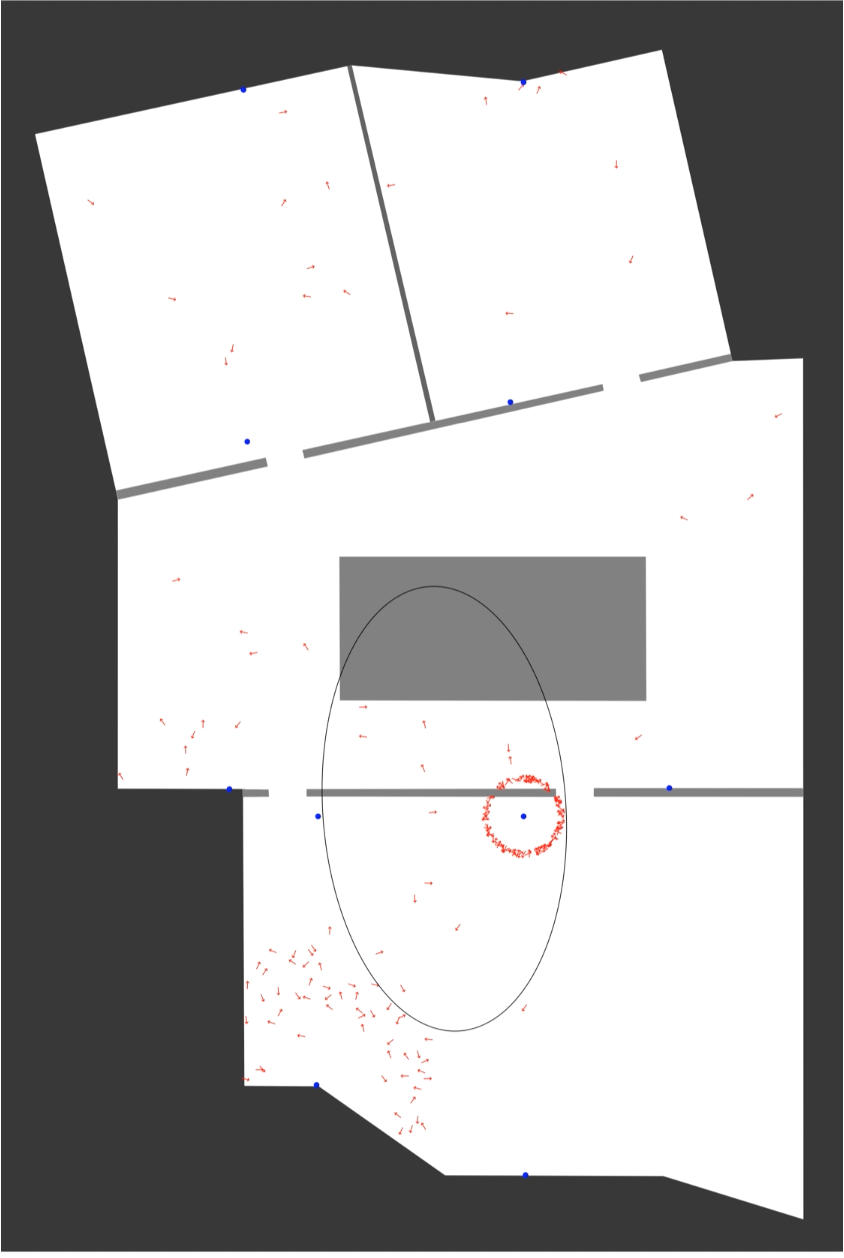
\includegraphics[height=0.7\textwidth]{figures/algo_particle_generation}
\caption{Depicts the initial posteriori belief, resp.\ the initial particle set. Particles are shown as red arrows, the beacons as blue filled circles. The large black circle is the $1\sigma$-ellipse.}
\label{fig:pf_initialDist}
\end{figure}

Before actually can start to continuously run our \acs{PF}'s implementation, we need to generate the initial posteriori belief $\chi_0$, resp.\ the particle set. As mentioned in chapter~\ref{chap:ibeacons}, each of the beacons can be uniquely identified by combining its three identifiers. In addition, we know the beacons, aka.\ landmarks, positions on the map. Consequently, we can use this information to specifically distribute the initial particles around the received beacons, which is a huge advantage instead of just uniformly distribute them on the map's free space. Therefor, our implementation starts ranging for beacons, and then wait's until \acl{CL} delivers the first set. Then, the particles are distributed in a circle around the beacons with radius of the estimated distance to the beacons. To take the distance estimations uncertainty into account, each distance of a particle to its beacon gets added some Gaussian noise $\sigma = 0.2 * d$, which depends on the estimated distance $d$. Additionally, the amount of particle being spread around a beacon depends also on the distance to it. $50\%$ of the particle set size are spread around the beacon, which is most probably the closest to the smartphone, according to the distance estimations. Around the second closest $25\%$, the third $12.5\%$, and so on. The last one gets the remaining particles. The particles are being generated with a random orientation $\theta$ where $\theta = [0, 2\pi)$. Figure~\ref{fig:pf_initialDist} shows a screenshot of our iOS app, depicting the initial particle set. The particles are depicted as red arrows and the beacons as blue filled circles. The black large circle shows the $1\sigma$~ellipse, which we are going to explain later on.


\subsection{Motion Integration}

% INTEGRATE MOTION
\begin{figure}
\begin{lstlisting}[mathescape]
integrateMotion($\chi_{t-1}$, $u_t$) {

  $\bar{\chi}_t = \emptyset$

  for $m = 1$ to $M$ {
    $x^{[m]}_t$ = sample_motion_model($u_t$, $x^{[m]}_{t-1}$)
  }
  
  return $\bar{\chi}_t$
}		
\end{lstlisting}
\caption{Helper function to apply the motion $u_t$ to the particle set $\chi_{t-1}$, by sampling from the motion model.}
\label{lst:pf_integrateMotion}
\end{figure}

The \texttt{integrateMotion} function, shown in figure~\ref{lst:pf_integrateMotion}, is a helper function to reduce the complexity of the later introduced algorithm. It gets passed the current particle set $\chi_{t-1}$ and the motion $u_t$ which it applies to each particle. Therefore, it samples from the motion models as discussed in section~\ref{sec:algo_sample_motion}. In the end, it returns the new particle set $\chi_t$.


\subsection{Filtering}

% FILTER
\begin{figure}
\begin{lstlisting}[mathescape]
filter($\chi_{t-1}$, $z_t$, map) {
  
  $\bar{\chi}_t = \emptyset$

  // importance factoring
  for $m = 1$ to $M$ {
    $w^{[m]}_t$ = measurement_model($z_t$,$x^{[m]}_t$, map)
    add $\langle x^{[m]}_t, w^{[m]}_t \rangle$ to $\bar{\chi}_t$
  }
  
  $\chi_t = \emptyset$
  
  \\ resampling
  while size of $\chi_t$ less $M$ {
    draw $i$ with probability $\propto w^{[m]}_t$
    add $x^{[i]}_t$ to $\chi_t$
  }
  
  return $\chi_t$
}		
\end{lstlisting}
\caption{Helper function for the importance factoring and resampling.}
\label{lst:pf_filter}
\end{figure}

Our \texttt{filter} function is another helper function, which is responsible for the \emph{importance factoring} and the \emph{resampling}, depicted in figure~\ref{lst:pf_filter}. It gets passed the particle set $\chi_{t-1}$, the measurements $z_t$ and the map. Then it determines the importance factor for each particle, as explained in section~\ref{sec:algo_measurement_model}. Afterwards, the resampling takes place to transform the old distribution into the new posteriori distribution, as described in section~\ref{sec:fund_pf}.

 The shown implementation is the basic implementation which does not solve the \emph{kidnapped robot} localization problem. To better understand our implementation, we reduce our \acs{PF}'s complexity, by first showing a simplified filter function, which neglects the recovery from failure state. Later in the chapter, we enhance the shown \texttt{filter} function, to explain our recovery feature. 

\subsection{\acl{PF}}
After explaining all prerequisites of our solution, we now give a detailed insight into our implementation of the \acl{PF}. To reduce complexity, we split up the \acs{PF}'s code into three logical parts, shown in figure~\ref{lst:algo_pf_1}, \ref{lst:algo_pf_2} and \ref{lst:algo_pf_3}. Figure~\ref{lst:algo_pf}, indicates their call order. It also contains several instance variables, which are accessible from the three parts.


\paragraph{Instance Variables} As already mentioned, the motions and measurements are asynchronously being delivered by their framework. Our motion model already reduces this problem by combining the two headings and the estimated walked distance, thus the \acs{PF}'s implementation has just to deal with two asynchronous sources. To overcome the asynchrony, the motions $u$ and measurements $z$ are buffered in two ascending ordered lists, the \texttt{u\_buffer} and \texttt{z\_buffer}, according their timestamps. The stored motions, resp.\ measurements, are provided by the motion model, resp.\ measurement model, and defined as described in section~\ref{sec:algo_motion_model}, resp.\ section~\ref{sec:algo_measurement_model}. The instance variable $u_\text{latest}$ stores, as the name already implies, the latest motion that was being calculated by the motion model. The \texttt{map} variable stores the environment's map in form of a occupancy grid and the landmarks, resp.\ the beacons, with their unique identifier and position on the map.

\paragraph{\texttt{particleFilter}} The \texttt{particleFilter} function is continuously, $\sim 1 \text{sec}$, being called if new measurements are available. To remember, \acl{CL} calls its delegate to update the ranged beacons, whether it received a beacon's signal, or not. Consequently, when the \texttt{particleFilter} function gets called, the latest measurements are always available and ready for processing. It gets passed the particle set $\chi_{t-1}$ and returns the set $\chi_t$.

\begin{figure}
\begin{lstlisting}[mathescape]
// instance variables
u_buffer // list of not jet integrated motions $u_t$
$u_\text{latest}$ // stores the latest motion
z_buffer // list of not jet integrated measurements $z^{[k]}_t$
map // occupancy grid and landmarks

particleFilter($\chi_{t-1}$) {

  $\bar{\chi}_t = \chi_{t-1}$

  $\bar{\chi}_t$ = PART_1($\bar{\chi}_t$)
  
  $\bar{\chi}_t$ = PART_2($\bar{\chi}_t$)
  
  $\bar{\chi}_t$ = PART_3($\bar{\chi}_t$)
    
  return $\chi_t$
}
\end{lstlisting}
\caption{Shows our \acs{PF}'s implementation and the used instance variables. To reduce the complexity the code is split up into three parts, shown in figure~\ref{lst:algo_pf_1}, \ref{lst:algo_pf_2} and \ref{lst:algo_pf_3}.}
\label{lst:algo_pf}
\end{figure}


\paragraph{Part 1} The algorithm's first part, shown in figure~\ref{lst:algo_pf_1}, consists of basically one loop, which tries to integrate the buffered motions and to filter with the buffered measurements at the right point in time. The loop is executed as long both buffers are not empty. The four if-cases are visualized in figure~\ref{fig:algo_pf_1}. In each example, the \texttt{u\_buffer} contains two motions $u_0, u_1$, and \texttt{z\_buffer} contains just $z_0$. Each subfigure illustrates just the first loop iteration, thus $u_1$ is not relevant during the iteration.

\textbf{Case 1} (fig.\ \ref{fig:algo_pf_1_1}): If a motion $u_0$ is in the buffer and also a measurement $z_0$ and the motion endet before the measurement was done ($u.{t_\text{end}} < z.t$), then the motion is being integrated and $z$ is reserved for the next iteration.

\textbf{Case 2} (fig.\ \ref{fig:algo_pf_1_2}): If a measurement was taken exactly at the end of a motion ($u.{t_\text{end}} = z.t$), than the motion is being integrated and afterwards the set can be filtered with the measurement.

\textbf{Case 3} (fig.\ \ref{fig:algo_pf_1_3}): If a measurement was taken during a motion ($u.{t_\text{start}} < z.t < u.{t_\text{end}}$), the motion needs to be split-up. The first sub motion can then be integrated into the set, which is afterwards being filtered. The second sub motion is put into the buffer at the first place, to be processed during the loop's next iteration.

\textbf{Case 4} (fig.\ \ref{fig:algo_pf_1_4}): If the measurement was taken before the motion ($u.{z.t < t_\text{start}}$ / \texttt{else}), the filter is being executed without integrating the motion. The motion is kept back for the next iteration.

If one of the buffers is empty, the algorithm continues with the second part.

% PART 1
\begin{figure}
\begin{lstlisting}[mathescape]
PART_1($\chi_{t-1}$) {

  $\bar{\chi}_t = \chi_{t-1}$

  while u_buffer isNotEmpty && z_buffer isNotEmpty {
    $u$ = u_buffer.first
    $z$ = z_buffer.first
    if $u.{t_\text{end}}$ < $z.t$ {
      $\bar{\chi}_t$ = integrateMotion($\bar{\chi}_t$, $u$)
      u_buffer.remove($u$)
    } else if $u.{t_\text{end}} = z.t$ {
      $\bar{\chi}_t$ = integrateMotion($\bar{\chi}_t$, $u$)
      $\bar{\chi}_t$ = filter($\bar{\chi}_t$, $z$, map)
      u_buffer.remove($u$)
      z_buffer.remove($z$)
    } else if $u.{t_\text{start}} < z.t$ && $z.t < u.{t_\text{end}}$ {
      split $u$ at timestamp $z.t$ in $u_1$ and $u_2$
      $\bar{\chi}_t$ = integrateMotion($\bar{\chi}_t$, $u_1$)
      $\bar{\chi}_t$ = filter($\bar{\chi}_t$, $z$, map)
      u_buffer.remove($u$)
      insert $u_2$ at beginning of u_buffer
      z_buffer.remove($z$)
    } else {
      $\bar{\chi}_t$ = filter($\bar{\chi}_t$, $z$, map)
      z_buffer.remove($z$)
    }
  }
  
  return $\bar{\chi}_t$
}
\end{lstlisting}
\caption{Part 1}
\label{lst:algo_pf_1}
\end{figure}

\begin{figure}
\subfloat[Case: $u.{t_\text{end}} < z.t$]{
	\begin{tikzpicture}
	  \draw[->] (0,1) -- (6,1);
  	  \draw (6.5,1)node(y){$t$};
  	    	  
  	  \draw[blue] (1,2)--(3,2);
  	  \draw[blue] (2,2.5)node(a){$u_0$};
  	  
  	  \draw[red, dashed] (3,2)--(5,2);
  	  \draw[red] (4,2.5)node(a){$u_1$};
  	  
  	  \draw (4,1)--(4,0.5);
  	  \draw (4,0)node(a){$z_0$};
	\end{tikzpicture}
	\label{fig:algo_pf_1_1}
}
\subfloat[Case: $u.{t_\text{end}} = z.t$]{
	\begin{tikzpicture}
	  \draw[->] (0,1) -- (6,1);
  	  \draw (6.5,1)node(y){$t$};
  	    	  
  	  \draw[blue] (1,2)--(3,2);
  	  \draw[blue] (2,2.5)node(a){$u_0$};
  	  
  	  \draw[red, dashed] (3,2)--(5,2);
  	  \draw[red] (4,2.5)node(a){$u_1$};
  	  
  	  \draw (3,1)--(3,0.5);
  	  \draw (3,0)node(a){$z_0$};
	\end{tikzpicture}
	\label{fig:algo_pf_1_2}
}

\subfloat[Case: $u.{t_\text{start}} < z.t < u.{t_\text{end}}$]{
	\begin{tikzpicture}
	  \draw[->] (0,1) -- (6,1);
  	  \draw (6.5,1)node(y){$t$};
  	    	  
  	  \draw[blue] (1,2)--(3,2);
  	  \draw[blue] (2,2.5)node(a){$u_0$};
  	  
  	  \draw[red, dashed] (3,2)--(5,2);
  	  \draw[red] (4,2.5)node(a){$u_1$};
  	  
  	  \draw (2,1)--(2,0.5);
  	  \draw (2,0)node(a){$z_0$};
	\end{tikzpicture}
	\label{fig:algo_pf_1_3}
}
\subfloat[Case: \texttt{else}]{
	\begin{tikzpicture}
	  \draw[->] (0,1) -- (6,1);
  	  \draw (6.5,1)node(y){$t$};
  	    	  
  	  \draw[blue] (1,2)--(3,2);
  	  \draw[blue] (2,2.5)node(a){$u_0$};
  	  
  	  \draw[red, dashed] (3,2)--(5,2);
  	  \draw[red] (4,2.5)node(a){$u_1$};
  	  
  	  \draw (0.5,1)--(0.5,0.5);
  	  \draw (0.5,0)node(a){$z_0$};
	\end{tikzpicture}
	\label{fig:algo_pf_1_4}
}
\caption{Visually illustrates the four cases shown in figure~\ref{lst:algo_pf_1}.}
\label{fig:algo_pf_1}
\end{figure}


\paragraph{Part 2} If after executing the first part, resp.\ after integrating all measurements, still motions are buffered, these motions are being integrated. Due to the fact, that the \texttt{particleFilter} function is being called if new measurements are being received, the buffered motions need to be older than the next, not jet occurred, measurement. Thus they can be integrated.

After integrating a motion, the filter method is being called. The filtering is being executed without a actual measurement. Thus just the map's occupancy grid is used for the importance factoring. Consequently, particles that are moved to a occupied position, are being sorted out.

The purpose of not just waiting for the next measurement resp.\ the particle filters call, to integrate the remaining motions is, that if the user is out of the beacons range, the motion is still being integrated, thus the particles on the view are still moving according to the users motion.

% PART 2
\begin{figure}
\begin{lstlisting}[mathescape]
PART_2($\chi_{t-1}$) {

  $\bar{\chi}_t = \chi_{t-1}$

  // integrate residual motions, filter just with map
  while u_buffer isNotEmpty {
    $u$ = u_buffer.first
    $z = \emptyset$
    $\bar{\chi}_t$ = integrateMotion($\bar{\chi}_t$, $u$)
     u_buffer.remove($u$)
     
     // filter without measurements, just with map
     $\bar{\chi}_t$ = filter($\bar{\chi}_t$, $z$, map)
  }
  
  return $\bar{\chi}_t$
}
\end{lstlisting}
\caption{Part 2}
\label{lst:algo_pf_2}
\end{figure}

\paragraph{Part 3}First two part are important for integrating and filtering during a person's walk. We found out, that integrating measurements if a person is stationary drastically can improve the estimated location accuracy. Therefor, we directly integrate the received measurements instead of buffering them, shown in figure~\ref{lst:algo_pf_3}. Thus, the user sees without a big latency how the posteriori changes by applying the measurements.

To be able to integrate them directly, we need to be sure that the person is stationary. As mentioned in chapter~\ref{chap:sensors}, \acs{CL} has the problem of requiring 6--8 steps to recognize that the person is walking, resp.\ until it delivers this information. Consequently, if a user is stationary and starts to walk, the measurements collected during the first steps need to be buffered until the motion data is available, otherwise the measurements would be integrated at the wrong position. The second important information is to know, that a person is now stationary, and no further motions are being delivered. Then, the measurements can directly be integrated.

The latter one can be solved easily. Motions are being delivered approx.\ every $2.5~sec$. Thus, if the difference between now and the latest motion $u_\text{latest}$ is at least $2.7~sec$, we can absolutely be sure, that \acs{CM} does not deliver any new motion until the person starts to walk again. $2.7~sec$ was chosen, because the $2.5~sec$ are an approximate value. Besides that the \texttt{particleFilter} function is just being called every $\sim1~sec$, thus no additional latency is being created.

To be able to buffer the measurements during the first steps when the user starts to walk again, we use the solution presented in section~\ref{sec:algo_stationary}. Due to the simple moving average over the last one second, we can detect within approx.\ one second if a user is stationary or not. If the user is not stationary, the integration is not being executed, thus the values are kept in the buffer.

Additionally, we found out, that applying a small Gaussian random motion with $\sigma = 0.3~m$ before applying the measurements, by filtering the particle set, helps to faster improve the location accuracy. If a person is stationary, the person's orientation does not matter. Consequently, also the motion's orientation $\theta$ is set randomly between $[0, 2 \cdot \pi)$. Using a random orientation has also the advantage, that the particles can move in any direction.

% PART 3
\begin{figure}
\begin{lstlisting}[mathescape]
PART_3($\chi_{t-1}$) {

  $\bar{\chi}_t = \chi_{t-1}$
  
  $\Delta t$ = currentDate - $u_\text{latest}.t_\text{end}$ // in seconds

  if motionModel.deviceIsStationary && $\Delta t \le 2.7$  {
    $u$ = motion with distance $0.0$
    $z$ = z_buffer.first
    
    $\bar{\chi}_t$ = integrateMotion($\bar{\chi}_t$, $u$)
    $\bar{\chi}_t$ = filter($\bar{\chi}_t$, $z$, map)
    z_buffer.remove($z$)
  }
  
  return $\bar{\chi}_t$
}
\end{lstlisting}
\caption{Part 3}
\label{lst:algo_pf_3}
\end{figure}


\subsection{Recovery / Kidnapping Problem}
Recovery has two purposes in our application. Firstly, it can happen, that all particles are moving out of bounds, and thus are being filtered out. Secondly, the particles are on a totally wrong position, which can happen if the user walked to soft, and thus, the pedometer could not recognize the users steps, or the orientation does not fit the actual one, because the user's phone pointed not straight forward during the walk.

To determine both situations, we enhanced our \texttt{filter} function shown in figure~\ref{lst:pf_filter}. The enhanced version is shown in~\ref{lst:pf_recovery}. During the resampling, the new particle set's $\texttt{weightSum} = \sum_{m = 0}^{M-1} w^{[m]}_t$, which is the sum of all drawn particles, during the resampling, is being calculated.

If the $\texttt{weightSum} == 0$, $\chi_t$ is empty, thus all particles are moved out of bounds or their location is already occupied and thus, they are being ignored. Consequently, a new random particle set is being generated. The particles are being distributed as described in section~\ref{sec:algo_initial}, in other words, the position estimation is restarted.

If the $\texttt{weightSum} > 0$, it gets normalized by the particle sets size. Then, it is being stored in an array \texttt{particleSums}, which contains the latest three weightSums (line 24). When the \texttt{filter} function gets called the next time, it first checks if the array already contains three weight sums, and if true, the average of the three weight sums is being calculated (line 8). If the average drops below a certain threshold ($1.0$), we know, that the posteriori's distribution does not match the user's true position, resp.\ it is totally wrong. To recover from this state we add additional $20\%$ random particles. The random particles are also being distributed as described in section~\ref{sec:algo_initial}. Due to the fact, that the particles are added before the importance factoring and resampling, the added particles should help to recover from the state, by getting higher importance factors, and thus are being drawn multiple times.

We tested different random particle counts, and $20\%$ seems to bring the best result. Adding to less particles does not really help to recover, but adding to much results in a heavily jumping position estimation. The reason for taking the average over the last three weight sums is, that it sometimes can happen, that the weight sum drastically drops during one filter call. This happens for instance, if the measurements to the beacons where heavily influenced, and thus totally wrong.

Figure~\ref{fig:algo_recovery} illustrates the recovery. The shown weight sums correspond to the two screenshots. During the experiment, we simulated the kidnapping problem, by walking very smooth from the lower lecture hall through the buildings foyer, by passing the large obstacle at the left side, into the upper right lecture hall. After being their stationary for a few seconds, we returned, by passing the obstacle on the other side. The walk's start and end are at the position, where the particles are being concentrated in figure~\ref{fig:algo_recovery_withRecovery}. During the walk, the iPhone's pedometer was not able to recognize any step. Both experiments, the one with recovery (fig.~\ref{fig:algo_recovery_withRecovery}) and the one without recovery (fig.~\ref{fig:algo_recovery_withoutRecovery}), are being simulated by using real recorded data as input.

We empirically found out, that a threshold of $1.0$ fits best. After $\sim 90~\text{sec}$ the recovery was being executed the first time. During the long break from $60 - 90~\text{sec}$, the walk through the foyer, no beacons, with an estimated distance less than $5~m$, where ranged. After, receiving measurements again, the average particle weight sum dropped below the threshold, and recovery took place. Thus, the particles jumped from the lower to the upper lecture hall. The same happened at $\sim 155~\text{sec}$ on the way back. The third recovery was being executed at $\sim 184~\text{sec}$, which caused the small jump to the end point.

With disabled recovery, we can see that the algorithm is not possible to find the true location. After $\sim 90~\text{sec}$ the weight sum drops to $\sim 0$ and stays there.


% FILTER
\begin{figure}
\begin{lstlisting}[mathescape]
// instance variable
weightSums // array that stores the last 3 weight sums

filter($\chi_{t-1}$, $z_t$, map) {
  
  $\bar{\chi}_t = \emptyset$
  
  if size of weightSum == 3 && avg.\ weightSums < 1.0 {
    add $0.2\%$ additional random particles to $\chi_{t-1}$ 
  }

  // importance factoring
  $\ldots$
    
  weightSum = $0.0$
  
  \\ resampling
  while size of $\chi_t$ less $M$ {
    $\ldots$
    weightSum += $w^{[m]}_t$
  }
  
  if weightSum > 0 { 
    override oldest value in weightSum with (weightSums/particleSetSize)
  } else {
    $\chi_t$ = generate new random particle set
    clear weightSums
  }
  return $\chi_t$
}		
\end{lstlisting}
\caption{Helper function for the importance factoring and resampling.}
\label{lst:pf_recovery}
\end{figure}

\begin{figure}
\subfloat{
	\begin{tikzpicture}
		\begin{axis}[trim axis left, trim axis right, width=0.9\textwidth, height=0.4\textheight,
			xlabel={Time (sec)},
			ylabel={ParticleWeightSum},
			legend entries={with recovery, without recovery},
			grid = major]
			\addplot [red, mark=x] table[col sep=semicolon, x=timestamp, y=normalizedWeightSum] {csv/F-Foyer2_F007-F023-F007_kidnapping/ParticleWeight_withRecovery.csv};
			\addplot [blue, mark=x] table[col sep=semicolon, x=timestamp, y=normalizedWeightSum] {csv/F-Foyer2_F007-F023-F007_kidnapping/ParticleWeight_withoutRecovery.csv};
		\end{axis}
	\end{tikzpicture}
}

\subfloat[with recovery] {
  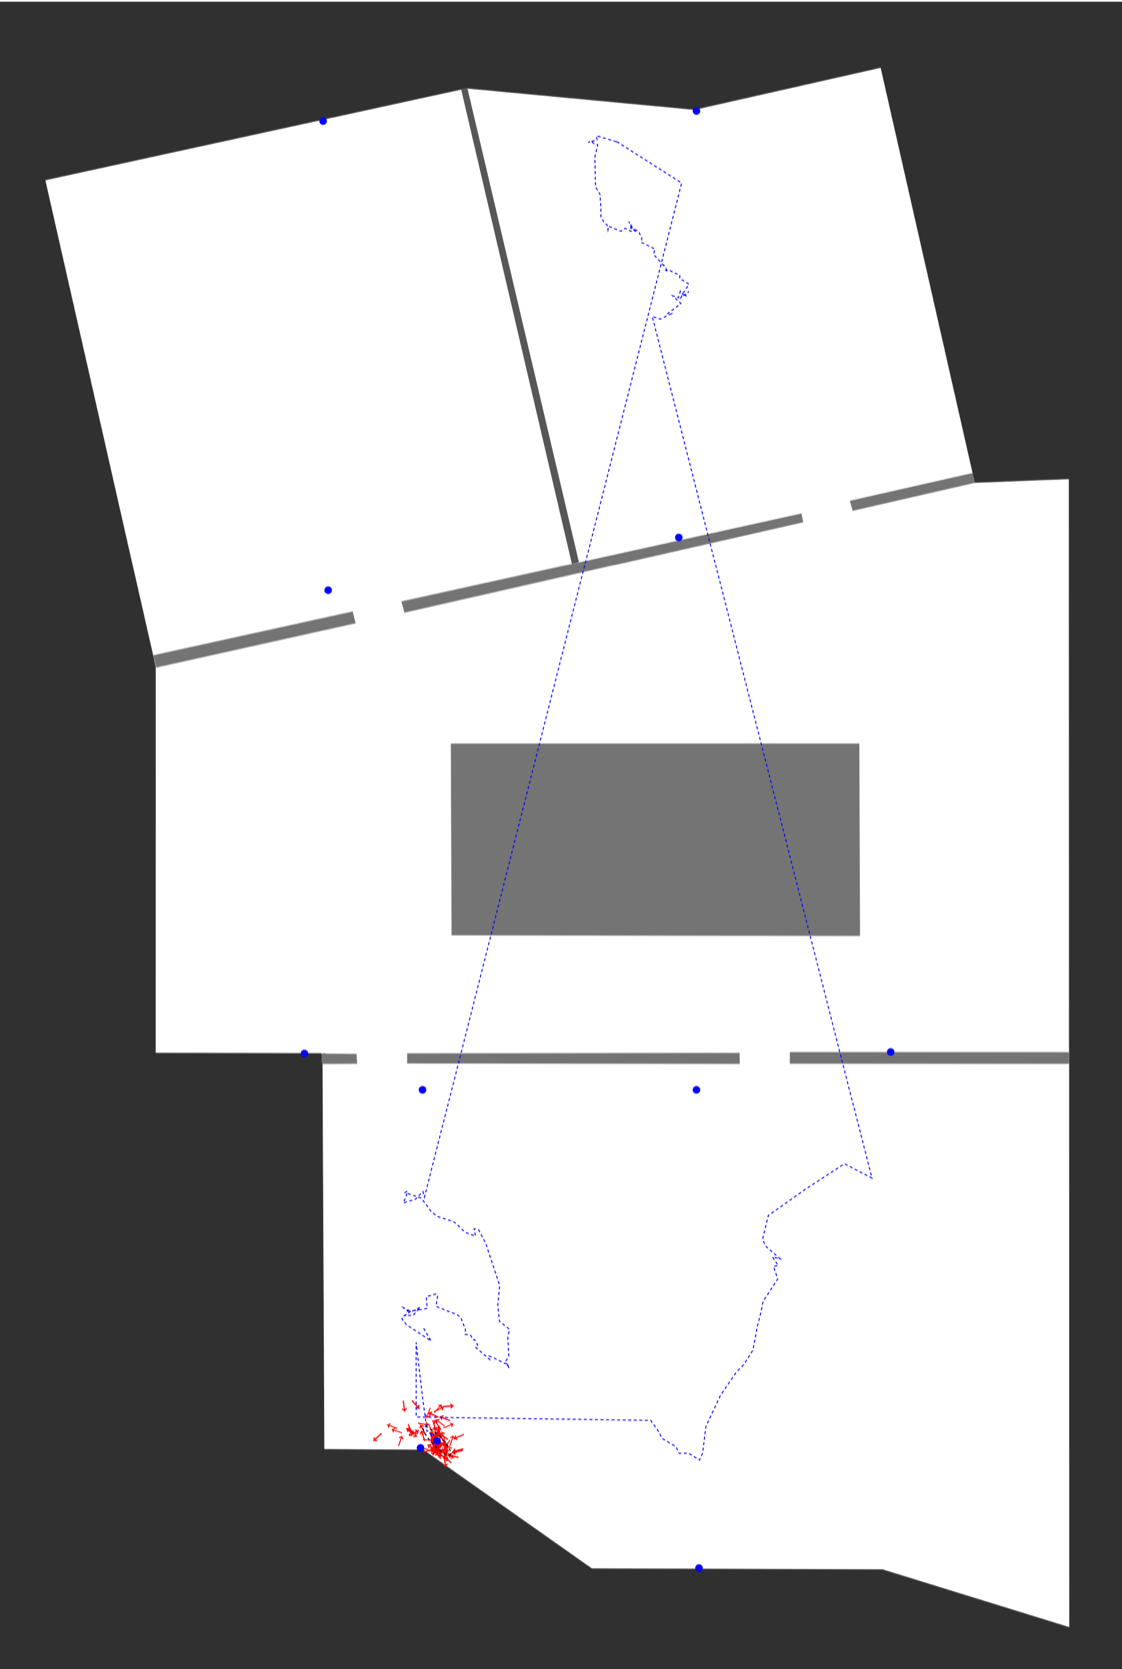
\includegraphics[height=0.5\textheight]{figures/algo_withRecovery}
  \label{fig:algo_recovery_withRecovery}
}
\subfloat[without recovery] {
  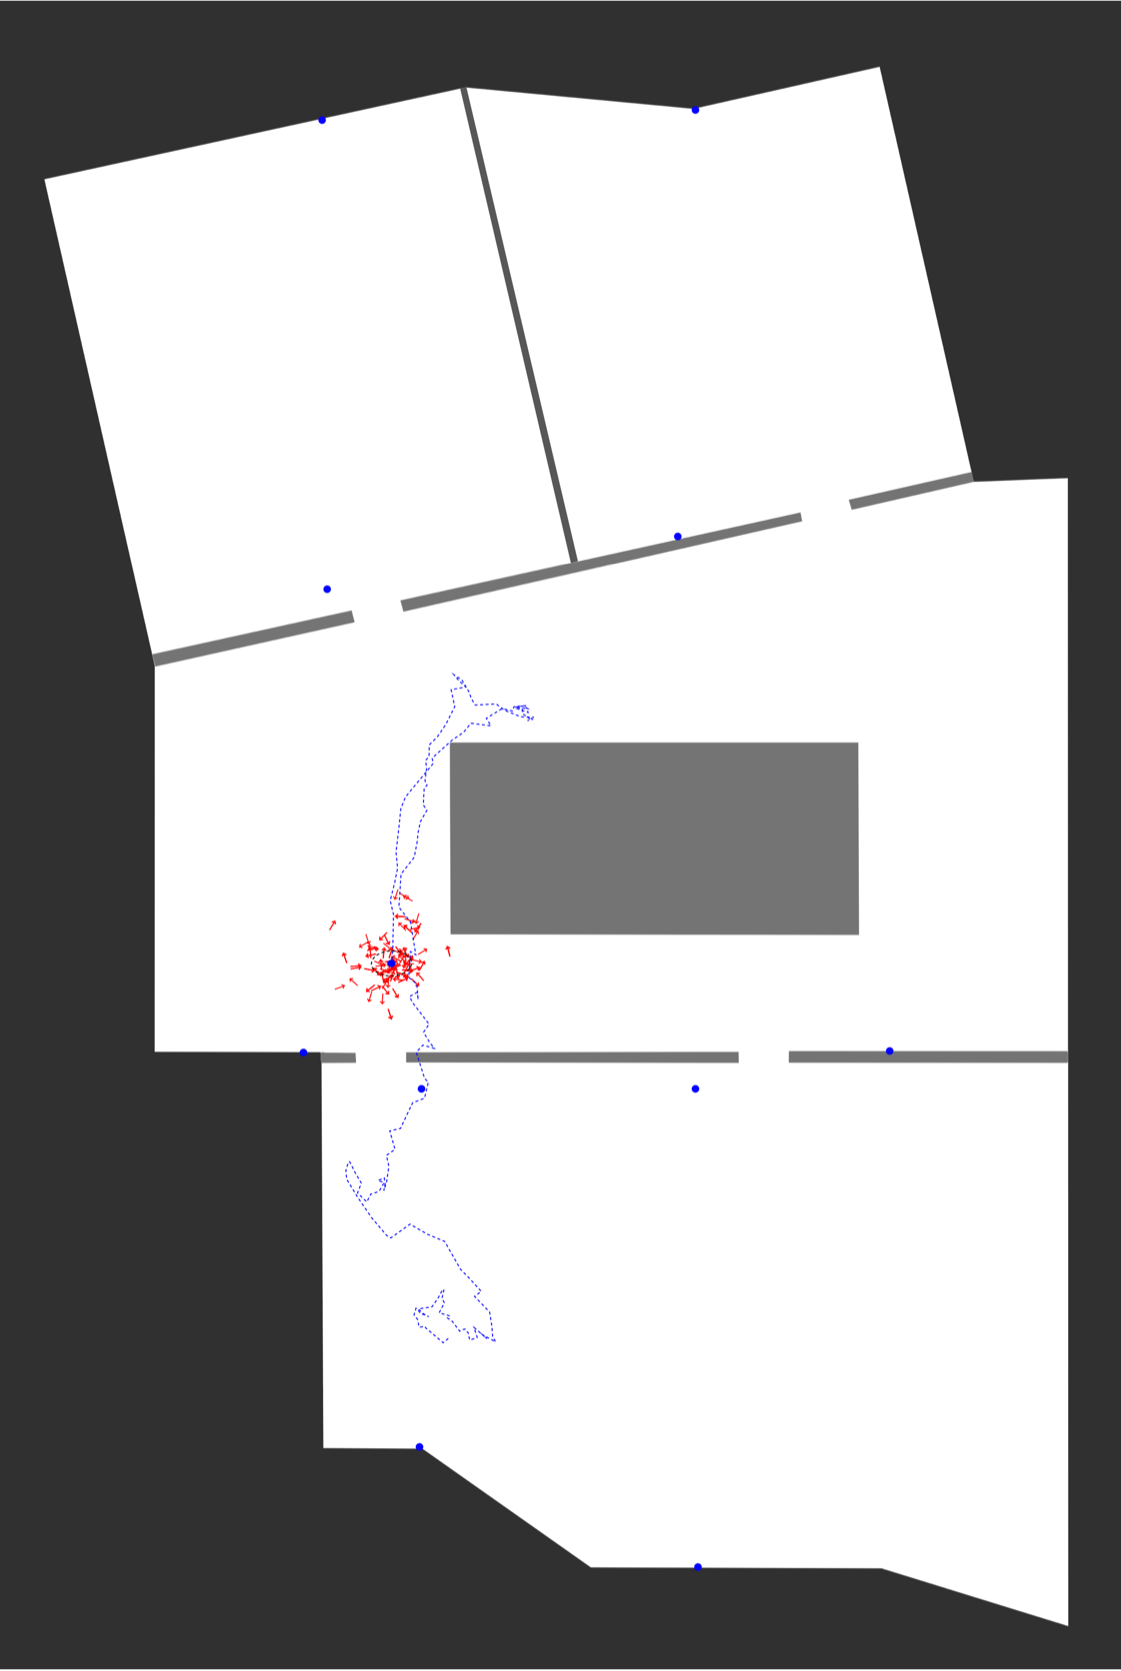
\includegraphics[height=0.5\textheight]{figures/algo_withoutRecovery}
  \label{fig:algo_recovery_withoutRecovery}
}
\caption {Depicts the build in recovery, which adds additional $20\%$ particles if the average weight sum drops below a threshold of $1.0$.}
\label{fig:algo_recovery}

\end{figure}

\subsection{Location Estimation}
To be able to display a concrete location estimation instead of a particle cloud, the \acs{PF}'s posteriori belief, which is a multi-modal distribution, represented by the particle set $\chi_t$, needs to be converted into another distribution. As mentioned in chapter~\ref{chap:fundamentals}, uncertainties are typically modeled as gaussians. Consequently, it is applicable to transform \acs{PF}'s posteriori into a two-dimensional gaussian $N(\mu, \Sigma)$, where the mean $\mu = (x, y)^T$ represents the concrete location, and the location's uncertainty is being expressed as the covariance matrix $\Sigma = \bigl(\begin{smallmatrix} \sigma_{x}^2&\sigma_{xy}\\ \sigma_{yx}&\sigma_{y}^2 \end{smallmatrix} \bigr)$.

The mean $\mu$, can either be $\chi$'s arithmetic mean or its weighted mean, by using the particle's importance factors as weights. Based on the estimated mean the covariance $\Sigma$ can be determined. The gaussian's parameters can then be used to visualize the user's location on the map in form of a $1\sigma\text{-ellipse}$, thus the user's true location is with a probability of $68\%$ somewhere in the $1\sigma\text{-ellipse}$. Figure~\ref{fig:algo_sigellipse}, depicts the transformation of the particle set $\chi$ into a gaussian, shown as $1\sigma\text{-ellipse}$.

\begin{figure}
	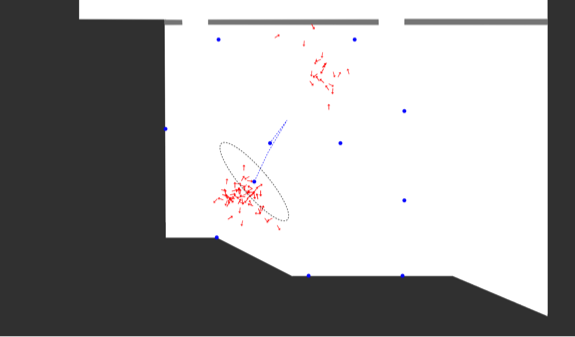
\includegraphics[width=0.7\textwidth]{figures/sigellipse}
	\caption{Depicts the transformation of $\chi$ into a gaussian, shown as $1\sigma\text{-ellipse}$, with a weighted mean.}
	\label{fig:algo_sigellipse}
\end{figure}
